\documentclass[11pt]{article}

\usepackage[italian]{babel}

\usepackage[utf8]{inputenc} % Required for inputting international characters
\usepackage[T1]{fontenc} % Output font encoding for international characters

\usepackage{mathpazo} % Palatino font
\usepackage{graphicx}
\usepackage{fancyhdr}
\usepackage{tabularx}
\usepackage{geometry}

\geometry{legalpaper, margin=2.5cm}

\newcommand{\doctitle}{System Design Document}
\newcommand{\docversion}{1.0}

\begin{document}
	
	%----------------------------------------------------------------------------------------
	%	TITLE PAGE
	%----------------------------------------------------------------------------------------
	
	\begin{titlepage} % Suppresses displaying the page number on the title page and the subsequent page counts as page 1
		\newcommand{\HRule}{\rule{\linewidth}{0.5mm}} % Defines a new command for horizontal lines, change thickness here
		
		\center % Centre everything on the page
		
		%------------------------------------------------
		%	Headings
		%------------------------------------------------
		
		\textsc{\LARGE Università degli Studi di Salerno}\\
		\textsc{\large Corso di Ingegneria del Software}\\[1.5cm] % Main heading such as the name of your university/college
		
		%------------------------------------------------
		%	Title
		%------------------------------------------------
		
		\HRule\\[0.4cm]
		
		{\huge\bfseries ASCETIC}\\ % Title of your document
		\vspace{0.2cm}
		{\large\bfseries Automated Code Smell Identification and Correction}\\[0.2cm] % Title of your document
		
		\HRule\\[1.5cm]
		
		\textsc{\Large \doctitle}\\[0.3cm] % Major heading such as course name
		
		\textsc{\large Version 1.1}\\[0.5cm] % Minor heading such as course title
		
		
		%------------------------------------------------
		%	Logo
		%------------------------------------------------
		
		\vfill\vfill
		
		
\includegraphics[width=0.5\textwidth]{Various/ascetic_logo.jpg}\\[1cm] % Include a department/university logo - this will require the graphicx package
		
		%------------------------------------------------
		%	Date
		%------------------------------------------------
		
		\vfill\vfill\vfill % Position the date 3/4 down the remaining page
		
		{\large\today} % Date, change the \today to a set date if you want to be precise
		
		
		
		%----------------------------------------------------------------------------------------
		
		\vfill % Push the date up 1/4 of the remaining page
		
	\end{titlepage}
	
	%----------------------------------------------------------------------------------------
	
	\pagestyle{fancy}
	\rhead{ASCETIC}
	\lhead{\doctitle~v.~\docversion}
	\renewcommand{\headrulewidth}{0pt}
	\textbf{Coordinatore Progetto:}
	\begin{table}[h]
		\centering
		\begin{tabularx}{0.9\textwidth}{|X|X|}
			\hline
			\textbf{Nome}     & \textbf{Matricola} \\ \hline
			Manuel De Stefano &  0522500633\\ \hline
		\end{tabularx}
	\end{table}

	\vspace{0.5cm}
	
	\textbf{Partecipanti:}
	\begin{table}[h]
		\centering
		\begin{tabularx}{0.9\textwidth}{|X|X|}
			\hline
			\textbf{Nome}     & \textbf{Matricola} \\ \hline
			Amoriello Nicola &  0512104742\\ \hline
			Di Dario Dario &  0512104758\\ \hline
			Gambardella Michele Simone &  0512104502\\ \hline
			Iovane Francesco &  0512104550\\ \hline
			Pascucci Domenico &  0512102950\\ \hline
			Patierno Sara &  0512103460\\ \hline
		\end{tabularx}
	\end{table}

	\textbf{Revision History:}
	\begin{table}[h]
		\centering
		\begin{tabularx}{0.9\textwidth}{|p{2cm}|l|X|p{3cm}|}
			\hline
			\textbf{Data} & \textbf{Versione} & \textbf{Descrizione} & \textbf{Autore} \\ \hline
			11/12/2018 & 1.0 & Prima stesura & Tutto il Team \\ \hline
			27/12/2018 & 1.1 & Ridefinite le interfacce dei sottosistemi & Tutto il Team \\ \hline
		\end{tabularx}
	\end{table}
	\newpage
	
	
	\tableofcontents
	\newpage
	
	 \section{ Introduction}
 
		\subsection{Purpose of the system}
		
			Durante il ciclo di vita di un software, le modifiche costituiscono una parte essenziale ed inevitabile. La manutenzione, volta alla correzione di bug o all'integrazione di nuove funzionalità, porta ad un graduale deperimento del codice, il quale non inficia il corretto funzionamento del software bensì introduce delle debolezze di progettazione: i cosiddetti Code Smell. Per questo motivo nasce ASCETIC, un plug-in sviluppato per l'IDE intelliJ IDEA che consente di analizzare il progetto, rilevando 4 possibili tipologie di smell(Blob, Promiscuous Package, Feature Envy, Misplaced Class), ed effettuare un'eventuale correzione automatica. \\ ASCETIC (inizialmente TACOR) è un'opera di reingegnerizzazione, ed offre allo sviluppatore la possibilità di: 
\begin{itemize}
	\item Identificare le quattro sopracitate tipologie di Code Smell.
	\item Correggere automaticamente i Code Smell trovati dal sistema. 
	\item Far ignorare al sistema determinati Code Smell, selezionati ad hoc dallo sviluppatore, trovati in fase d'analisi. 
	\item Porre nella sezione "To do" di IntelliJ, tramite la funzione Reminder, gli Smell che lo sviluppatore decide di correggere manualmente in un secondo momento. 
\end{itemize}
Allo stato attuale ASCETIC usufruisce di una tecnica di analisi testuale per il rilevamento dei vari Code Smell: il primo step consiste nell'estrazione del contenuto testuale che caratterizza le componenti del codice, facendo una cernita degli elementi necessari per l'analisi, ossia i commenti e gli identificatori. Questi ultimi vengono normalizzati, ed infine le parole normalizzate vengono pesate in base allo schema tf-idf. Le componenti normalizzate vengono analizzate dallo Smell Detector, basato su LSI, che trasforma le componenti del codice in vettori di termini presenti in un dato software.  Tali vettori vengono proiettati in un K-spazio , ridotto appositamente per limitare l'effetto del rumore testuale. La dimensione di tale spazio viene determinata usando l'euristica di Kuhn. Infine la somiglianza fra i documenti viene calcolata come il coseno dell'angolo tra i due vettori. I valori vengono calcolati in maniera differente a seconda dello Smell da individuare per ottenere le probabilità che la porzione di codice sia affetta da tale Smell. Tali probabilità vengono convertite in valori booleani per indicare se un componente sia affetto o meno da Code Smell e richieda quindi una correzione. La scelta di questo metodo è dettata sia dalla validità comprovata di tale tecnica, sia dalla mancanza momentanea di alternative valide per effettuare il procedimento svolto dal plug-in in fase d'analisi. Uno degli obiettivi di sviluppo però è rendere ASCETIC flessibile alle modifiche ed all'introduzione di eventuali nuove tecniche per la gestione dell'analisi del codice. Per quanto riguarda il procedimento di refactoring, ASCETIC utilizza le API di IntelliJ per la manipolazione del codice sorgente. 

			
		\subsection{Design goals}
		
			L'operazione di reengineering del plug-in ASCETIC dovrà tenere conto di un'alta manutenibilità, in modo che l'utente possa inserire con facilità nuove funzioni di analisi e correzione.
\\
Il reengineering apporterà anche modifiche sul piano dell'usabilità, con un'interfaccia gradevole e intuitiva.
\\
Il plug-in dovrà effettuare le operazioni richieste in tempi accettabili, con bassi consumi di memoria e in assenza di output errati.
\\
Inoltre i casi di crash o blocchi dovrà essere ridotta al minimo e in caso di errori dovrà essere in grado di segnalare il problema e mostrare all'utente istruzioni per un'eventuale risoluzione.
\\
Il sistema continuerà ad essere implementato completamente in Java e continuerà ad avere un modesto livello di sicurezza, poiché l’esecuzione viene svolta completamente in locale e non memorizza dati sensibili degli utenti.
\\
Di seguito verranno elencati i criteri di qualità ricavati dai requisiti non funzionali.

\subsubsection{Performance Criteria}

		\begin{tabular}{|p{3cm}|p{13cm}|}
		\hline
		
		\vfill \centering \textbf{Tempi di risposta} \vfill & \vfill Il sistema deve essere reattivo, ma gran parte di questo dipende dalla mole di dati da elaborare e dalle prestazioni del dispositivo usato.\vfill \\ \hline 			
		\vfill \centering \textbf{Throughput} \vfill & \vfill Il sistema tiene conto del tempo impiegato per una singola istruzione piuttosto che del numero di correzioni effettuabili in parallelo\vfill \\
		\hline
		\vfill \centering \textbf{Memoria} \vfill & \vfill Il sistema memorizza i dati persistenti in file distinti su memoria locale. E' implementata una meccanica di caching volta ad accelerare il recupero dei dati, che derivano dall'analisi testuale del codice, la quale è computazionalmente onerosa. \vfill \\
		\hline
		
		\end{tabular}
	
\subsubsection{Dependability Criteria}

		\begin{tabular}{|p{3cm}|p{13cm}|}
			\hline
			
			\vfill \centering \textbf{Robustezza} \vfill & \vfill Il sistema restituisce sempre un output che rispecchia le aspettative dell'utente. Cioè, nel caso in cui è possibile restituire una soluzione valida, il sistema la esegue. Nel caso in cui si verifichi un errore oppure non sia possibile restituire una soluzione valida, il sistema notificherà l'insuccesso all'utente. \vfill \\ 
			\hline 			
			\vfill \centering \textbf{Affidabilità} \vfill & \vfill Il sistema non deve essere soggetto a frequenti casi di crash. In caso ciò accada il sistema deve essere in grado di notificare all'utente di eventuali input errati. \vfill \\
			\hline
			\vfill \centering \textbf{Disponibilità} \vfill & \vfill Il sistema è disponibile all'uso dell'utente in qualsiasi momento dall'avvio dell'ambiente di sviluppo IntelliJ. \vfill \\
			\hline
			\vfill \centering \textbf{Tolleranza all'errore} \vfill & \vfill Il sistema è in grado di riconoscere un possibile disservizio e gestirlo notificando l'errore all'utente e salvando i progressi fatti fino al guasto. \vfill \\ 
			\hline 			
			\vfill \centering \textbf{Sicurezza} \vfill & \vfill Il sistema è usufruibile da qualsiasi utente che utilizza il plug-in perché non vengono memorizzati dati sensibili. Gli unici dati memorizzati sono parti di codice da rielaborare. \vfill \\
			\hline
			
		\end{tabular}

\subsubsection{Cost Criteria}

		\begin{tabular}{|p{3cm}|p{13cm}|}
			\hline
			
			\vfill \centering \textbf{Costi di sviluppo} \vfill & \vfill È stimato un costo complessivo di 4800 ore per la progettazione e lo sviluppo del sistema (80 ore per ogni membro del team). \vfill \\
			\hline 			
			\vfill \centering \textbf{Costi di amministrazione} \vfill & \vfill È stimato un costo complessivo di 40 ore per l'amministrazione del sistema (40 ore per ogni PM del team). \vfill \\
			\hline
			
		\end{tabular}

\subsubsection{Maintenance Criteria}

		\begin{tabular}{|p{3cm}|p{13cm}|}
			\hline
			
			\vfill \centering \textbf{Estensibilità} \vfill & \vfill Il sistema è progettato in modo tale da poter essere esteso con altre funzionalità oppure ampliare la tipologia di smell che possono essere analizzati/corretti con le funzionalità già presenti. \vfill \\
			\hline 			
			\vfill \centering \textbf{Modificabilità} \vfill & \vfill Il codice è stato scritto secondo paradigmi ingegneristici. Il tutto è stato scritto seguendo una specifica suddivisione in moduli, i quali rendono la struttura leggibile e intuitivamente modificabile. \vfill \\
			\hline
			\vfill \centering \textbf{Adattabilità} \vfill & \vfill Il plug-in funziona su qualsiasi sistema operativo purché sia provvisto dell'applicativo IntelliJ IDEA. Non sarà possibile utilizzarlo su IDE diversi da questo (Eclipse, Visual Studio, NetBeans,...). \vfill \\
			\hline
			\vfill \centering \textbf{Leggibilità} \vfill & \vfill Il sistema sarà fornito di una documentazione esauriente che avvalora la leggibilità della struttura del codice. \vfill \\
			\hline 			
			\vfill \centering \textbf{Portabilità} \vfill & \vfill La portabilità è garantita dalla scelta implementativa adoperata, giacché Java è per sua natura un linguaggio votato alla portabilità. \vfill \\
			\hline
			\vfill \centering \textbf{Tracciabilità dei requisiti} \vfill & \vfill La tracciabilità dei requisiti sarà possibile, si può retrocedere al requisito associato ad ogni parte del progetto. La tracciabilità sarà garantita dalla fase di progettazione fino al testing. \vfill \\
			\hline
			
		\end{tabular}

\subsubsection{End user Criteria}

		\begin{tabular}{|p{3cm}|p{13cm}|}
			\hline
			 			
			\vfill \centering \textbf{Utilità} \vfill & \vfill Il sistema si rivela utile poiché in assenza di questo l'utente avrebbe impiegato sforzi e tempi maggiori, oltre ai possibili errori di distrazione che a un occhio umano potrebbero sfuggire. \vfill \\
			\hline
			\vfill \centering \textbf{Usabilità} \vfill & \vfill L'interazione fra il sistema e l'utente sarà molto semplice anche senza la consultazione della documentazione associata. L'interfaccia risulterà intuitiva e gradevole da usare, sia per novizi che per esperti. \vfill \\
			\hline
			
		\end{tabular}
	
\subsubsection{Trade-off}
	
		\begin{tabular}{|p{3cm}|p{13cm}|}
			\hline
			
			\textbf{Trade-off} & \\
			\hline
			
			\vfill \centering Manutenibilità \\ vs \\ Performance \vfill  & \vfill Il reenginering del sistema da priorità alla manutenibilità suddividendo il codice del progetto in più moduli coerenti con le proprie finalità. Questa preferenza favorisce la leggibilità del codice per future operazioni di manutenzione, ma può gravare sensibilmente sulle performance. \vfill \\
			\hline
			\vfill \centering Performance \\ vs \\ Memoria \vfill  & \vfill Il reenginering del sistema da priorità alla performance. L'algoritmo di analisi viene eseguito una sola volta all'avvio del software per poi memorizzare i risultati in memoria primaria e secondaria tramite una meccanica di caching. Solo in caso di modifiche al codice verrà rieseguito l'algoritmo di analisi per aggiornare la cache e se queste sono effettuate su i file originali verrà rieseguito il caching anche sulla memoria persistente.  \vfill \\
			\hline
			\vfill \centering Performance \\ vs \\ Sicurezza \vfill  & \vfill Il reenginering del sistema da priorità alle performance a discapito della sicurezza, poiché l'obiettivo del plug-in è quello di ridurre i tempi di lavoro dei vari utenti nella risoluzione di code smell. La sicurezza viene trascurata perché non vengono manipolati dati sensibili. \vfill \\
			\hline
			\vfill \centering Manutenibilità \\ vs \\ Sicurezza \vfill & \vfill Il reenginering del sistema da priorità alla manutenibilità del plug-in. In questo modo l'utente può ampliare l'elenco di smell e aggiungere nuove funzionalità. Siccome sarà possibile mettere mano al codice, il livello di sicurezza può essere messo a rischio. \vfill \\
			\hline
			\vfill \centering Usabilità \\ vs \\ Sviluppo rapido \vfill & \vfill Il reenginering del sistema da priorità all'usabilità del plug-in, realizzando una nuova e intuitiva interfaccia con la quale l'utente può interagire in modo rapido. Tuttavia i costi in termine di tempo di sviluppo aumentano. \vfill \\
			\hline
			\vfill \centering Robustezza \\ vs \\ Portabilità \vfill & \vfill Il reenginering del sistema da priorità alla robustezza del plug-in, il quale dovrà restituire in ogni caso l'output sperato dall'utente. Il sistema è compatibile solo con l'ambiente di sviluppo IntelliJ IDEA.\vfill \\
			\hline
			
		\end{tabular}	
				
		\subsection{Definitions, acronyms, and abbreviations}
		
			Code Smell : porzioni di codice scritte in maniera non ottimale, le quali non compromettono il funzionamento del sistema ma introducono debolezze di progettazione, riducendo la qualità complessiva del codice. \\
TACOR : acronimo per Textual Analysis for Code smell detectiOn and Refactoring. \\
ASCETIC : acronimo per Automated Code Smell Identification and Correction. \\
tf-idf : abbreviazione di term frequency inverse document frequency. \\
LSI : abbreviazione di Latent Semantic Indexing. \\


		
		\subsection{References}
		
			Si fa riferimento :
\begin{itemize}
	\item al libro "Object-Oriented Software Engineering- using UML, Pattern and Java Bernd Bruegge Allen H.Dutoit"
	\item ai precedente documentazione riguardante il progetto.
\end{itemize}
	
	\section{Current software architecture}
	
			Il sistema corrente presenta una \textit{three-tier architecture} in cui sono presenti i classici 3 layer: \textit{presentation}, \textit{application} e \textit{storage}. 

\begin{figure}[h!]
	\centering
	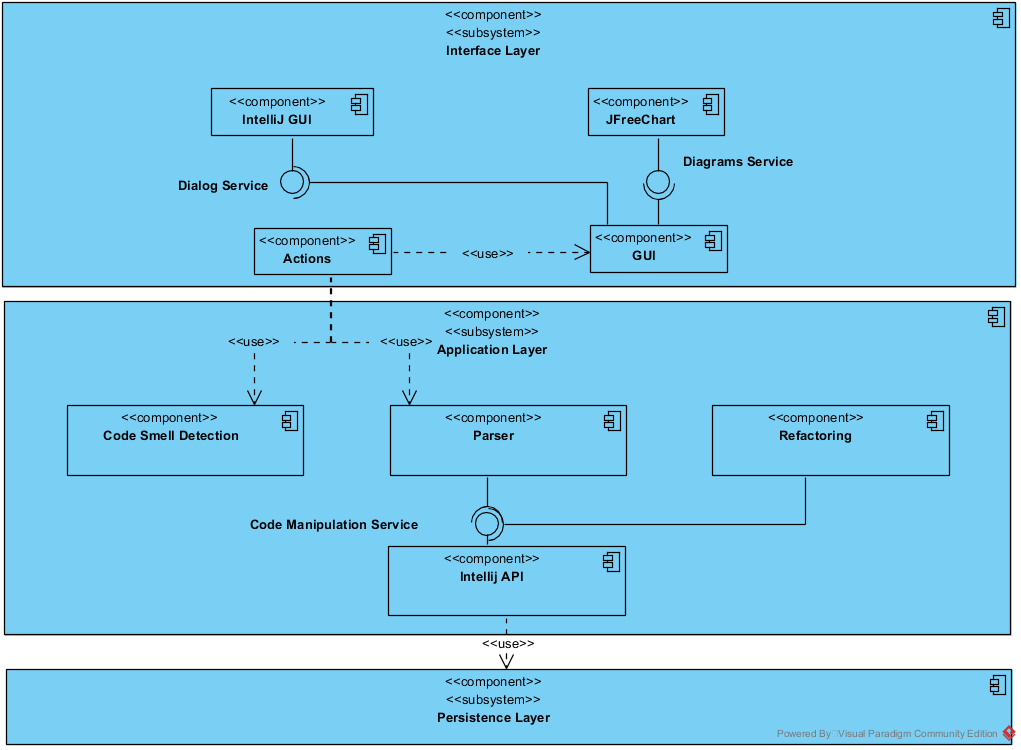
\includegraphics[scale=0.7]{./CS_Architecture/Diagrams/TACOR-Component.png} \\
	\textbf{Current Architecture Overview}
\end{figure}


\paragraph{}Il \textit{presentation layer} include tutte le interfacce grafiche e le \textit{actions}, ovvero componenti che, opportunamente configurate, eseguono codice in risposta a interazioni dell'utente con componenti grafiche estese dell'IDE. Queste componenti fungono, dunque, da connettori tra Intellij e il codice del plugin.

\paragraph{} L' \textit{application layer} contiene tutto il codice di business del plugin ed è composto da 3 componenti principali: \textit{Code Smell Detection}, \textit{Parser} e \textit{Refactoring}. Il primo si occupa delll'individuazione dei code smell all'interno dei componenti codice sotto analisi, il secondo di ricavare dal codice in esame le informazioni necessarie al \textit{Code Smell Detection} per effettuare le analisi, mentre il terzo si occupa di mettere in atto le operazioni di refactoring correttive dei \textit{code smell}. Tutti e tre sono utilizzati e coordinati dalle classi \textit{actions} e dagli \textit{action listeners} delle interfacce grafiche e quindi utilizzati come se fossero un \textit{Service Layer} che agisce su classi che mantengono solamente dati, i beans. Tutto ciò indica che il plugin presenta un'architettura, come la definisce Martin Fowler, \textit{anemica}.

\paragraph{} Lo \textit{storage layer}, invece, è costituito dai files contenente il codice sorgente in esame. Esso non viene mai acceduto direttamente dal codice di business del plugin, ma attraverso le API offerte dalla piattaforma Intellij.

\paragraph{} Le modifiche presenti nella sezione 3 consistono in una rimodulazione e ristrutturazione generale dell'architettura, volte a risolvere i problemi di manutenibilità e la mancata adesione all'object-orientation che derivano dall'architettura anemica del sistema. Inoltre, tale ristrutturazione rende più semplice l'aggiunta delle due nuove funzionalità di correzione di \textit{Blob} e \textit{Promiscuous Package}. Per ulteriori dettagli, si fa riferimento al documento di \textit{Change Impact Analysis}.  
		
	\section{Proposed software architecture}	
		\subsection{Overview}
		
			


Le funzionalità del sistema verranno suddivise in component e layer logici in base alle differenti caratteristiche di queste. Sarà garantita massima coesione e minimo accoppiamento tra i sottosistemi in modo che i cambiamenti in un sottosistema non influiscano sugli altri.\\
Il sistema userà il modello architetturale MVC: impianto di memorizzazione (Model), presentazione (View) e business logic (Controller).
		
		\subsection{Subsystem decomposition}
		
			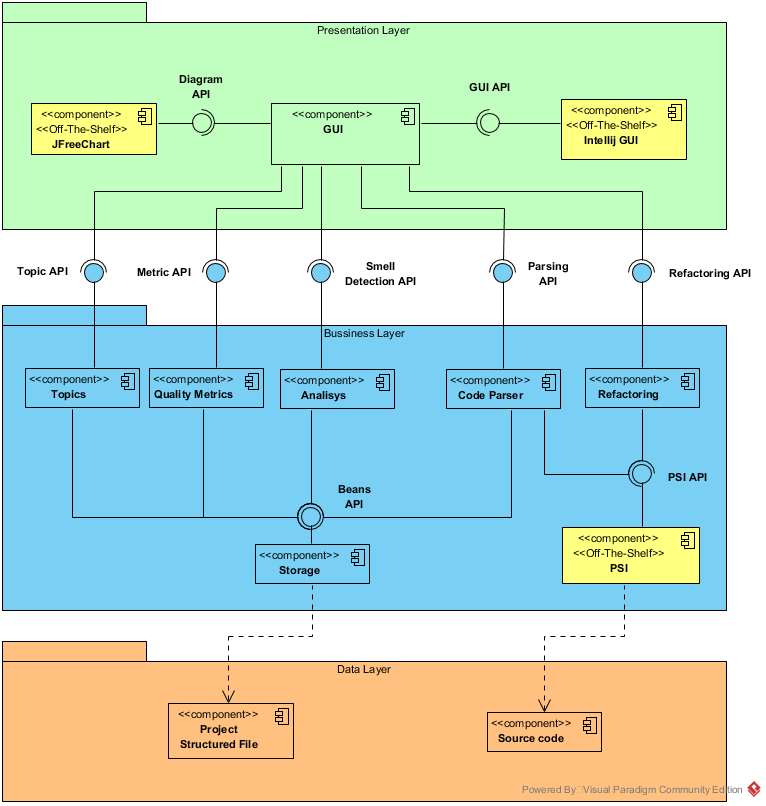
\includegraphics[scale=0.85]{PS_Architecture/diagrams_PNG/Component_Diagram.png}\\
\centering
\textbf{Component Diagram}\\

\flushleft

\begin{tabular}{|l|p{13cm}|}
	\hline
	\textbf{\Large Name} & \textbf{\Large Descrizione} \rule[-1cm]{0mm}{2cm} \\ \hline
	
	\textbf{Analisi} &  Componente che si occupa di analizzare il codice java identificando, tramite metriche e topic ottenute da altre componenti, la presenza di code smell.
	\rule[-1cm]{0mm}{1cm} \\ \hline
	\textbf{Refactoring} & Componente che si occupa di generare una possibile soluzione ad un code smell selezionato presente all'interno del codice java in analisi, procedendo poi all'eventuale applicazione di quest'ultima risolvendo così il code smell identificato. 
	\rule[-1cm]{0mm}{1cm} \\ \hline
	\textbf{Storage} & Componente gestisce l'accesso al file strutturato del progetto in analisi
	\rule[-1cm]{0mm}{1cm} \\ \hline
	\textbf{GUI} & Componente che realizza l'interfaccia grafica, la quale si appoggia su Intellij API(per componenti grafiche) e JFreeChart(per grafici). 
	\rule[-1cm]{0mm}{1cm} \\ \hline
	\textbf{Code Parser} & Componente che prende la struttura elaborata dal PSI come input ed, estrapolando informazioni da questo, costruisce i Beans fornendo così una diversa rappresentazione strutturata dell'input.
	\rule[-1cm]{0mm}{1cm} \\ \hline
	\textbf{Quality Metrics} & Componente che si occupa del calcolo delle metriche qualitative quali LOC, WNC, RFC, CBO, LCOM, NOA, NOM, NOPA e NOP.
	\rule[-1cm]{0mm}{1cm} \\ \hline
	\textbf{Topics} & Componente che si occupa del calcolo dei topic ovvero dei termini più ricorrenti all'interno del codice analizzato.
	\rule[-1cm]{0mm}{1cm} \\ \hline	
	\textbf{Project Structured File} & Componente che implementa una meccanica di cache realizzata in SQLite come singolo DB di cache per ogni progetto (descritta nel dettaglio nella sezione del Persistent data management).
	\rule[-1cm]{0mm}{1cm} \\ \hline	
\end{tabular}


			
		\subsection{Hardware/software mapping}
	
			



Il sistema sottoposto a reenginering sarà installato sull'ambiente di sviluppo IntelliJ IDEA e utilizzerà la libreria SQLite. Poichè il sistema è embedded il collegamento con gli altri sottosistemi è gestito dall'IDE nel quale in plug-in viene eseguito.
			
		\subsection{Component Off-The-Shelf}
		
			I componenti "off-the shelf" che useremo sono elencati di seguito, per i dettagli implementativi e, i motivi delle scelte si rimanda alla sezione API-Engineer e Trade-Off.
\\
\begin{itemize}
\item \textbf{IntelliJ GUI} : La GUI che realizzeremo si appoggerà su API di Sistema a mezzo API di IntelliJ.
\item \textbf{PSI (Program Structure Interface)} :
\begin{itemize} 
	\item \textbf{Code Manipulation API} : Il modulo di Refactor tramite queste API fornite da IntelliJ, effettua l'Extract e il Move per l'elaborazione delle smells sulle classi o sui package.
	\item \textbf{Compiler Services} : Il codice preso in esame dovrà sottoporsi al test di compilazione in modo tale da verificarne la correttezza lessicale, semantica e sintattica.
\end{itemize}

\item \textbf{JFreeChart (DiagramAPI)} : Libreria Java che offre servizi grafici (grafici a barre, Istogrammi,  a torta, grafico a radar). Nel nostro caso sarà utilizzato per rappresentare le RadarMap che rappresenteranno le topic implementate dalle varie componenti analizzate.
\end{itemize}
	
		\subsection{Persistent data management}	
		
			In ASCETIC la persistenza dei dati è necessaria soprattutto per tenere traccia di informazioni importanti ai fini delle funzioni offerte dal sistema. ASCETIC infatti deve essere in grado di: memorizzare le informazioni temporali relative all'ultima modifica del progetto, ricordare la struttura di quest'ultimo, ossia memorizzare quali e quanti smell vi sono all'interno. Queste caratteristiche rendono più semplice ed immediato il chaching che il sistema sfrutta per mantenere un certo standard in materia di performance. La principale Data Source di ASCETIC è costituita dunque dal codice sorgente del programma preso in esame su IntelliJ: il sistema non sfrutta quindi un vero e proprio DBMS, nonostante l'utilizzo di SQLite (scelto per motivi di ottimizzazione implementativa), ma associa ad ogni progetto un file contenente le informazioni di cui sopra. Lo schema di seguito riportato non costituisce un diagramma ER, bensì uno schema logico rappresentativo del come i file verranno strutturati mediante SQLite.

\hspace{1cm}

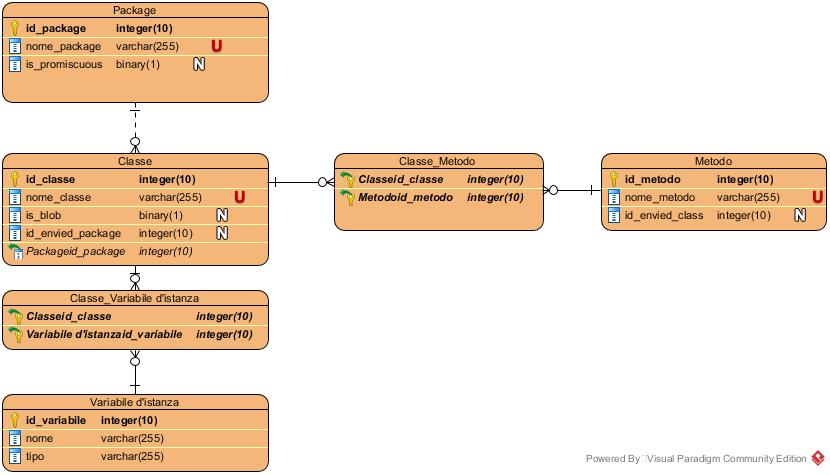
\includegraphics[width=1\textwidth]{Various/schema_logico.jpg}
			
		\subsection{Access control and security}
		
			


ASCETIC è un sistema basato su singolo utente. Chiunque abbia accesso alla macchina su cui è installato il plug-in può usufruire di tutte le sue funzionalità, che nello specifico sono:

	\begin{quote}
	
	\begin{itemize}
		
		\item Analisi
		
		\item Correzione
		
		\item Ignora correzione
		
		\item Ricorda azione
		
	\end{itemize}
	\end{quote}

Non viene adottata alcuna tipologia di politica di sicurezza, poiché il plug-in è accessibile da un solo tipo di attore e non sono presenti dati personali che possano essere danneggiati.
		
		
		\subsection{Global software control}
		
			


All'avvio del plug-in, un thread di controllo inizia la sua attività di analisi dell'intero progetto, creando, nel caso in cui sia stato effettuato il primo avvio, la cache. Per avvii successivi del plug-in, la cache viene aggiornata dal thread.
\\
Il controllo del flusso è gestito da classi di tipo controller poiché il sistema è basato su architettura MVC. Il sistema utilizzerà un controllo di flusso event-driven perché le azioni saranno innestate da eventi tramite interazioni dell'utente con l'interfaccia grafica (button, menù, ...). Quindi la gestione del flusso converge tutta su un'entità controller, la quale smisterà le differenti azioni al componente adatto a svolgerle.
		
		\subsection{Boundary conditions}
		
			Le condizioni limite riguardano solo ed esclusivamente il caso in cui il sistema dovesse andare in crash, poiché i casi relativi all'accensione ed allo spegnimento dipendono dall'avvio e dall'arresto di IntelliJ.   
\subsubsection{Crash Sistema} 
Il caso di crash del sistema (dovuto a qualche malfunzionamento del plug-in) viene gestito in modo tale che il sistema mostri i log all'utente e successivamente ne effettui la distruzione insieme alla cache . Così facendo l'utente è costretto a rieffettuare le operazioni precedenti al crash.  
 
\begin{tabular} {|l|p{11cm}|} 
  
 \hline 
 \textbf{ID} & \textbf{CRASH} \\ \hline   
\textbf{Participating actors}  & Sviluppatore \\ \hline 
 \textbf{Entry Condition} & Lo Sviluppatore sta utilizzando ASCETIC su IntelliJ \\ \hline 
 \textbf{Flow of events} &  
  \begin{tabular}{p{5cm} p{5cm} p{5cm}} 
   \centering \textbf{UTENTE} & \centering \textbf{SISTEMA}  & \\ 
   \textbf{1.}\hspace{0.3cm}L'utente, durante l'utilizzo del plug-in, riscontra un crash del sistema dovuto ad un errore casuale. & &  \\ 
   & \textbf{2.} \hspace{0.3cm}Il sistema mostra un messaggio d'errore. Successivamente, alla ripresa del normale funzionamento, mostra i log degli errori riscontrati  dopodiché procede all'invalidazione delle cache. & \\ 
   \textbf{3.}\hspace{0.3cm}L'utente prende visione delle notifiche del sistema e si appresta ad utilizzare di nuovo il plug-in, avendo cura di rieffettuare le operazioni precedenti al crash non soggette a salvataggio. & &  
  \end{tabular} 
 \\ \hline 
 \textbf{Exit condition} & Il sistema riprende a funzionare correttamente e sono state invalidate le cache. \\ \hline 
 \textbf{Exception condition} & \\ \hline 
 \textbf{Quality requirements} & \\ \hline  
\end{tabular}
		
	\section{Subsystem services}
	
		
\centering

\begin{tabular}{|l|l|l|l|}
	\hline
	\textbf{\Large Name} & \textbf{\Large Servizi offerti} & \textbf{\Large Servizi richiesti} &\textbf{\Large Dipendenze} \rule[-1cm]{0mm}{2cm} \\ \hline
	
	\textbf{Analisi} & Smell Detectors API & Persistence API & \\&& Beans API &  \rule[-0.5cm]{0mm}{0cm}   
	\rule[-0.5cm]{0mm}{0cm}
	\\ \hline
	\textbf{Refactoring} & Refactoring API & PSI API & \rule{0mm}{0.5cm}    
	\rule[-0.5cm]{0mm}{0cm}
	\\ \hline
	\textbf{GUI} & & GUI API & \rule{0mm}{0.5cm}\\&& Diagram API & \\&& Metric API & \\&& Topic API & \\&& Smell Detectors API &
	\\&& Parsing API & \\&& Refactoring API & \rule[-0.5cm]{0mm}{0cm}
	\\ \hline
	\textbf{Code Parser} & Parsing API & Beans API & \rule{0mm}{0.5cm} \\&& PSI API & 
	\rule[-0.5cm]{0mm}{0cm}
	\\ \hline
	\textbf{Quality Metrics} & Metric API & Beans API &  \rule{0mm}{0.5cm} \rule[-0.5cm]{0mm}{0cm}
	\\ \hline
	\textbf{Topics} & Topic API & Beans API & \rule{0mm}{0.5cm} \rule[-0.5cm]{0mm}{0cm}
	\\ \hline
	\textbf{Storage} & Beans API &  & Project Structured File\rule{0mm}{0.5cm} \rule[-0.5cm]{0mm}{0cm}
	\\ \hline
	\textbf{Project Structured File} &  &  & \rule{0mm}{0.5cm} \rule[-0.5cm]{0mm}{0cm}
	\\ \hline
	
\end{tabular}

\flushleft

\begin{itemize}
	\item \textbf{Beans API} : Permette la gestione dei Beans, fornendo così una rappresentazione ulteriormente strutturata del codice in analisi.
	\item \textbf{Smell Detectors API} : Analizza testualmente il codice strutturato in Bean, individuando i vari tipi di code smell (Feature envy, Misplaced class, Blob, Promiscue package).
	\item \textbf{Parsing API} : Esegue l'operazione di avvio dell'analisi con il conseguente riempimento del file. 
 	\item \textbf{Refactoring API} : Esegue l'operazione di refactoring del codice analizzato in seguito alla generezione di una possibile soluzione, da parte del sistema o dell'utente dove concesso. 	
	\item \textbf{Metric API} : Implementeremo una meccanica di calcolo e rilevamento di varie metriche qualitative utili all'analisi della porzione di codice designata.
	\item \textbf{Topic API} : Implementeremo una meccanica di rilevamento di topic quali termini più ricorrenti utili all'analisi della porzione di codice designata.
	
\end{itemize}




	
	\section{Glossary}
	
		
\begin{itemize}
	   			
	   			\item \textbf{Blob:} Tipoligia di code smell. E' una Classe che implementa responsabilità molto diverse tra di loro.
	   			
	   			\item \textbf{Feature Envy:} Tipoligia di code smell. E' un Metodo che è maggiormente interessato a variabili e metodi di una classe differente dalla sua.
	   			
	   			\item \textbf{IntelliJ IDEA:} IntelliJ IDEA è un ambiente di sviluppo integrato per il linguaggio di programmazione Java. E' stato sviluppato da JetBrains.
	   			
	   			\item \textbf{Misplaced Class:} Tipoligia di code smell. E' una Classe che non ha alcuna attinenza con le classi dello stesso package.
	   			
	   			\item \textbf{Promiscuous Package:} Tipoligia di code smell. E' un Package contenente classi che hanno responsabilità diverse.
	   			
	   			\item \textbf{TACOR:} Acronimo per Textual Analysis for Code smell detectiOn and Refactoring. E' un plug-in, sviluppato per l'IDE IntelliJ IDEA, creato per risolvere il problema dei "code smell" mediante l'analisi testuale. Esso è il progetto su cui è basato ASCETIC.
	   			
\end{itemize}
		
\end{document}